\documentclass[11pt]{article}

\usepackage[utf8]{inputenc}
\usepackage[T1]{fontenc}
\usepackage[francais]{babel}
\usepackage{fancyhdr}
\usepackage[scale=0.7]{geometry}
\usepackage{siunitx}
\usepackage{amsmath}
\usepackage{graphicx}
\usepackage{hyperref}
\usepackage{tabularx}
\usepackage[table]{xcolor}% http://ctan.org/pkg/xcolor



\pagestyle{fancy}
\renewcommand{\footrulewidth}{1pt}
\fancyfoot[C]{\textbf{page \thepage}}
\fancyfoot[L]{Polytech Nantes}
\fancyfoot[R]{2016 -- 2017}
\fancyhead[L]{Équipe 13}
\fancyhead[R]{INFO4}

\title{Mini-projet de C++ : Google Hashcode 2016\\Rapport de l'équipe 13}
\author{Vincent \bsc{Cotineau} \and Anthony \bsc{Griffon} \and Benjamin \bsc{Landry} \and Hugo \bsc{Pigeon} \and Pierre \bsc{Pétillon}}

\makeatletter
\let\ps@plain\ps@fancy
\makeatother

\hypersetup{
    pdftitle={Mini-projet de C++: Google Hashcode 2016},%
    pdfauthor={Equipe 13},%
    pdfsubject={C++},%
    pdfcreator={LaTeX},
    pdfproducer={Equipe 13},
    pdfkeywords={equipe 13, c++, hashcode, 2016}
}


\begin{document}
	% \begin{center}
	% \noindent\makebox[\textwidth][c]{%
	% \begin{minipage}[t]{0.7\textwidth}
	%   \begin{flushleft}
	%     
\includegraphics [width=100mm]{images/poly.png} \\[0.5cm]
	%   \end{flushleft}
	% \end{minipage}}
	% \end{center}
	% \let\newpage\relax%
	\maketitle
	
	Ce projet pose un problème complexe, qui demande une certaine réflexion pour arriver à un résultat donnant un score élevé. Il faut également faire attention à la façon d'implémenter la méthode de résolution, pour que le traitement se fasse le plus rapidement possible. Cela conduit à faire des choix de modélisation, qui ont une grande influence sur les algorithmes développés et donc sur le temps de calcul.
	
	Pour résoudre le problème posé, nous avons choisi de développer un algorithme naïf, simple à implémenter, afin d'avoir une première solution correcte. Pour améliorer les résultats obtenus et le temps de traitement, nous avons réfléchi en parallèle à un algorithme plus complexe. Dans ce rapport, nous allons présenter ces différents algorithmes.

	\section{Algorithme naïf}
		
			Le but de cette solution est d'obtenir un premier résultat à partir d'un principe relativement simple. Nous avons effectué quelques optimisations pour minimiser le temps de calcul, mais ce n'était pas l'objectif prioritaire de cette solution.
	
		\subsection{Principe}
			
			Le principe est donc le suivant : chaque satellite prend la photo la plus proche qu'il peut atteindre. Ainsi, on traite les satellites un par un, chacun effectuant ses déplacements sur toute la simulation en dirigeant en permanence sa caméra vers la prochaine photo qu'il peut prendre. Pour trouver la prochaine photo à prendre, on simule le déplacement du satellite sur chaque tour. On calcule à chaque fois la fenêtre de coordonnées que la caméra peut atteindre et on vérifie si une photo se trouve dans cette fenêtre. Si c'est le cas, que la photo n'a pas déjà été prise et qu'il est possible de la prendre au tour courant, alors on arrête la recherche. Sinon, on continue à simuler le déplacement du satellite, jusqu'à trouver une photo ou jusqu'à arriver à la fin du temps imparti. Une fois que la prochaine photo a été trouvée, on exécute réellement le déplacement du satellite, en dirigeant la caméra vers les coordonnées de la photo trouvée.
		
		\subsection{Optimisation}
		
			Afin d'accélérer l'exécution de cet algorithme, nous avons mis au point une optimisation qui diminue grandement le temps de traitement, sans changer le résultat. Ainsi, nous avons choisi d'utiliser le principe de la recherche dichotomique pour trouver rapidement la prochaine photo à prendre. En effet, il s'agit de la partie la plus longue du programme : avec une recherche séquentielle, pour chaque satellite on parcourt toutes les images à chaque tour.
			
			Le principe est donc d'avoir une liste de toutes les images, que l'on trie selon leur latitude puis selon leur longitude. A partir de là, on peut faire une recherche dichotomique sur la latitude, ce qui permet d'arriver rapidement à une image dont la latitude est dans la fenêtre de la caméra. On sait alors que les images qui se situent dans la fenêtre, si elles existent, sont classées autour de celle que l'on vient de trouver. On fait alors une recherche séquentielle sur toutes ces images proches jusqu'à en trouver une qui est dans la fenêtre, ou jusqu'à ce que l'on sorte de celle-ci.
			
			Il n'est cependant pas possible d'effectuer une recherche dichotomique pour trouver directement l'image de manière systématique avec ce principe. En effet, dans certains cas la recherche dichotomique peut supprimer de son espace de recherche des images dont la latitude est dans la fenêtre. Par exemple, si on arrive sur une image dont la latitude est correcte mais la longitude est trop grande, la recherche dichotomique considère que toutes les images dont la latitude est supérieure à celle-ci ne sont pas dans la fenêtre. Or c'est faux dans la plupart des cas : on peut avoir une image dont la latitude est supérieure mais toujours dans la fenêtre et dont la longitude est aussi dans la fenêtre.
			
	\section{Algorithme amélioré avec utilisation d'un ratio}
	
		Le but de cet algorithme est d'utiliser les différentes informations que nous avons sur les collections d'images à savoir le nombre de points à gagner, le nombre de tours et le nombre d'images à photographier. Ainsi, nous nous servons de ces informations pour créer une priorité sur les photos à prendre.
	
		\subsection{Principe}
		
		Le principe de cet algorithme est de se baser sur la solution naïve présentée précedemment en améliorant l'ordre de la sélection des photos à prendre pour les satellites. Ainsi, pour chaque satellite on identifie pour chaque tour, tout d'abord une photo ayant un ratio (NbPoints/NbPhotosAPrendre) supérieure et on la prend en photo si elle existe. Si tel n'est pas le cas, on choisit la photo la plus proche et on continue au prochain tour à trouver la photo la plus valable en moyenne.
		
		\subsection{Détails d'implémentation}
		
		Tout comme l'algorithme naïf, nous avons une liste de toutes les images du jeu de données. Cependant, nous choisissons d'abord de les trier via le ratio calculé pour chaque image avec un rapport entre le nombre de points de la collection et le nombre de photos à prendre. Si nous sommes dans un cas d'égalité de ratio, nous trions les images par leur latitude et leur longitude.
		
		Une fois la liste d'images triées, nous recherchons la meilleure image possible à prendre selon le ratio avec un intervalle de tours limité. Ainsi, on vérifie si la meilleure image n'a pas une distance de tours relativement élévée grâce à un seuil. Si tel est le cas, on vérifie si il n'existe pas d'autres photos plus proche. S'il n'y a pas de photos comprise dans le seuil de tours, on incrémente le tour afin de trouver une solution.
		
		Cependant, cet algorithme n'est malheureusement pas idéal car il se base sur l'hypothèse que la photo la plus valable permet de trouver le chemin le plus valable. Pour améliorer cet algorithme, il faudrait pouvoir comparer les chemins au fur et à mesure de l'avancée de l'algorithme et modifier le chemin à chaque fois que l'on en trouve un qui est plus intéressant. 

		% subsection résultats (end)

	\section{Nombre d'occurences} % (fold)
	\label{sec:encore_un_autre_algorithme}

	\subsection{Principe} % (fold)
		\label{sub:principe}
	Dans cette algorithme, on va retrouver les principes de l'algorithmes naïfs avec une implémentation différente. On va retrouver la notion de ratio vu d'un point de vue différent. On va supposer que le ratio: $r=\frac{nombreDOccurenceEnCours}{nombreDOccurenceTotal}$ (où le nombre d'occurence en cours correspond au nombre de fois où la photo a été vu par un satellite et le nombre d'occurence total le nombre de fois qu'elle peut être vu par l'ensemble des satellites) va décider de la prise d'une photo à la place d'une autre.
	\\
	\\
	On suppose ici que si on doit choisir entre deux photos, il vaut mieux prendre celle au ratio le plus élevé, et donc le nombre d'occurence restante le moins important maintenant.


	\subsection{Implémentation} % (fold)
		\label{sub:principe}
		Le principe est simple, il s'agit encore une fois de faire une boucle sur les satelittes, pour chaque satellites on va faire un tableau qui va lister toutes les photos qui peuvent être prises, qui va donner un nombre d'occurence pour chaque photo.
		\\
		\\
		Concernant l'implémentation, chaque satellite va disposer de ces deux vecteurs:
		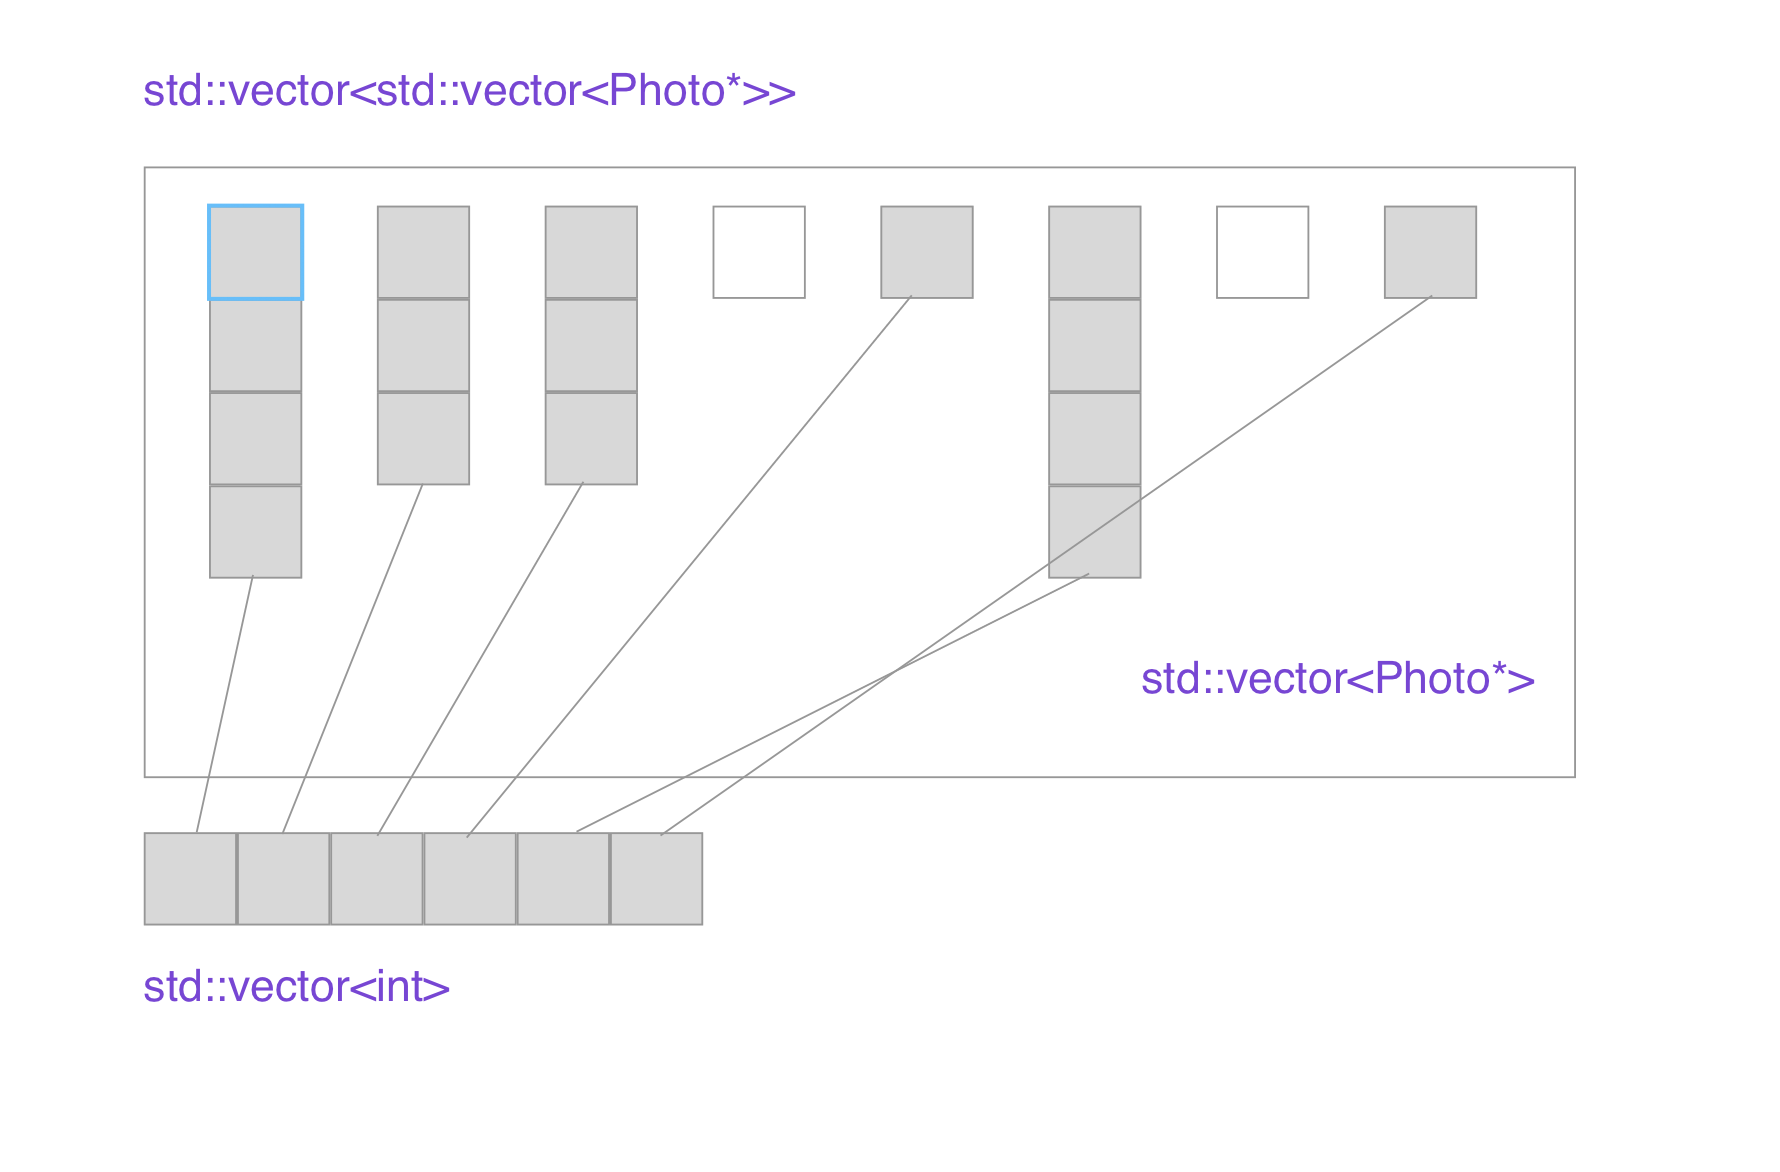
\includegraphics [width=100mm]{images/ex1.png} \\[0.7cm]
		Un vecteur de vecteur de photos, qui va contenir le vecteur de toutes les photos qui peuvent être prise par le satelitte tour par tour et un vecteur qui va indiquer les vecteurs non vide du précédent tableau.
		\\
		Une fois cela fait, on va commencer une simulation ou pour chaque satellite, on va faire l'ensemble des tours, et on va choisir quelle photo il prend plutôt qu'une autre en fonction du ratio.
		
	\subsection{Limites de l'algorithme} % (fold)
	\label{sub:limites_de_l_algorithme}

		L'algorithme est limité dans le fait ou il va regarder pour chaque satellite les uns après les autres, ce qui est un problème sur la façon dont nous avons conçu l'algorithme à la base, il faudrait en effet changer cette méthode car elle n'est pas la plus efficiente: le programme ne sait pas comment vont réagir les autres satellites ni comment ils vont tourner à ce stade, et donc les choix ne sont forcément pas les meilleurs.
		\\
		\\
		Une meilleure approche peut consister à augmenter les résultats en changeant l'ordre des satelittes ou refaire la simulation avec tous les ordres possibles et choisir le meilleur résultat. Le problème c'est que cela nécessite pour n satellites de lancer $n!$ fois la simulation.

	\section{Résultats} % (fold)
	\label{sec:résultats}
	
	% section résultats (end)

			\footnotesize
		\hspace*{-1cm}\noindent\begin{tabularx}{16cm}{|l|p{4cm}|X|p{2cm}|r|}
			\hline
			 & \textbf{Jeu de données} & \textbf{Temps} & \textbf{Score} & \textbf{Pourcentage} \\
			\hline
		    \cellcolor{blue!25} Algorithme 1 & & & & \\
		    \cellcolor{blue!25} & forever\_alone & X secondes & 44000 & 35.5 \\
		    \cellcolor{blue!25} & constellation & X secondes & 44000 & 35.5 \\
		    \cellcolor{blue!25} & overlap & X secondes & 44000 & 35.5 \\
		    \cellcolor{blue!25} & weekend & X secondes & 44000 & 35.5 \\
		    \hline
				\cellcolor{yellow!25} Algorithme Ratio & & & & \\
		    \cellcolor{yellow!25} & forever\_alone & X secondes & 48000 & 34.44 \\
		    \cellcolor{yellow!25} & constellation & X secondes & 64313 & 2.15 \\
		    \cellcolor{yellow!25} & overlap & X secondes & 14114 & 1.21 \\
		    \cellcolor{yellow!25} & weekend & X secondes & 50612 & 0.75 \\
				\hline
			\cellcolor{green!25} Algorithme occurences & & & & \\
		    \cellcolor{green!25} & forever\_alone & 1.21 secondes & 48000 & 34.44 \\
		    \cellcolor{green!25} & constellation & 83 secondes & 64313 & 2.15 \\
		    \cellcolor{green!25} & overlap & X secondes & 14114 & 1.21 \\
		    \cellcolor{green!25} & weekend & X secondes & 50612 & 0.75 \\
				\hline
		    \cellcolor{red!25} Meilleurs résultats & & & & \\
		    \cellcolor{red!25} & forever\_alone & X secondes & 44000 & 35.5 \\
		    \cellcolor{red!25} & constellation & X secondes & 44000 & 35.5 \\
		    \cellcolor{red!25} & overlap & X secondes & 44000 & 35.5 \\
		    \cellcolor{red!25} & weekdend & X secondes & 44000 & 35.5 \\
		    \hline
		\end{tabularx}
		\normalsize

	\section{Arbitre} % (fold)
	\label{sec:arbitre}
	


	% section arbitre (end)
	
	% subsection résultats (end)
	
	% subsection limites_de_l_algorithme (end)

		% subsection principe (end)	
	% section encore_un_autre_algorithme (end)

\end{document}
